\chapter{Preliminaries}\label{chapter:background}


{\color{red} related works
      about 4-6 pages

      make a distinction between methods/papers that discuss similar approaches and methods/concepts used in this thesis}

{ \color{red}

    about 20-30 pages (rather less I guess?)

    \begin{enumerate}
        \item Introduction to XAI in general
        \item Evaluation of XAI methods in general
        \item Structural Causal Models and causal framework
    \end{enumerate}
}

\section{Neural Networks}
Among the many machine learning approaches that have been developed, the most popular but also most opaque are deep neural networks. In general, a neural network consists of neurons, which are computational nodes organized in layers. In a forward pass, each neuron creates a weighted sum of its inputs, offsets it with a bias and then feeds it through a non-linear function. The result is fed to the next layer of neurons until the output layer is reached. During training, a loss function between the output for a data instance and its true label is optimized by back-propagating its gradient and updating the weights and biases. For specifics on successful architectures and training procedures we refer to text books on deep learning, for example by Goodfellow et al. \cite{Goodfellow2016}. When trained with enough data the weights and biases together approximate an often highly non-linear function describing the training data accurately. This function however is hard to analyze and interpret for humans, trying to understand the reasoning of the network. Hence the emergence of many explanation methods attempting to uncover those inner workings in a human-interpretable way.


\section{The Field of Explainable Artificial Intelligence}
With the field of machine learning and particularly complex deep neural network models ever expanding, so is the demand for explanations of these models.
As especially neural networks are so called \textit{black boxes} that inhibit a human understanding of their results, plenty of explanation methods have been developed, summarized under the term \textit{explainable AI} or short \textit{XAI}. 
\todo{more on why XAI is necessary in general}
\todo{post-hoc vs. interpretable models vs. ?}
Those methods can generally be divided into local and global approaches. While local methods aim to explain the decision making for one specific example, for example in computer vision tasks one image, typically by attributing importance to input features like pixels, global methods make more general interpretations of a model, for example, which features are identified in the decision-making process. The first category prominently includes saliency map methods \todo{cite}, which are most often tested on computer-vision tasks, where they assign importance to pixels or regions of a sample image, creating a heatmap. The importance is in most cases computed through forms of back-propagation \todo{cite} or with the help of gradients \todo{cite}. The resulting saliency maps may generate insight into the locality of important objects, however this is usually only one facet of understanding the decision-making, especially for people not familiar with the data domain.

\subsubsection{Local Attribution Methods}
\begin{itemize}
    \item what are local attribution methods?
    assign importance to each input feature
    most prominently used for computer vision tasks
    roughly divided into model-agnostic and backpropagation methods
    backpropagation further parted into gradient based and modified back-propagation methods
    \item common problems with local attribution methods: what is 100\%?
    what is a good explanation and what does "pixel is important" really tell us
    need not only where but also what is important about pixel
    therefore concept-based approaches got introduced
    \item lead over to more specifically just backgpropagation methods
\end{itemize}


\subsection{Backpropagation Methods}
GuidedBP, RectGrad, DTD, LRP (with different rules), PatternAttribution, DeepLIFT, Gradient, gradientXinput, Integrated Gradients...?

other modified backpropagation algorithms, everything that can be justified/ theoretically by taylor decomposition stuff
tell more about taylor decomposition?

\todo{LRP and surroundings: also other applications like pruning (if you can "prune" certain neurons, their causal effect must be none or extremely small \cite{Yeom2019})}

interpretation techniques based on backpropagation methods or building on top of them: 
\textit{activation maximization, feature attack (generative approaches), activation atlas, specific local and global models ... }


\todo{more overview papers and map of XAI papers}
categorization \cite{Samek2021}


\subsubsection{Layer-wise Relevance Propagation}
Layer-wise relevance propagation \cite{Bach2015} is the basis for concept relevance propagation and is among the most highly cited local attribution methods in XAI. Being introduced almost 10 years ago, it has been justified theoretically with Deep Taylor Decomposition \cite{Montavon2017}. It belongs to the class of (modified) back-propagation methods which propagate a custom value instead of a gradient back to the input. A visual representation of this strategy can be found in \cref{fig:crp_vs_lrp} \textbf{(a)}. As other saliency methods, LRP is commonly used in computer vision tasks to attribute importance to each pixel in an image, which can then be visualized as a heatmap, but is also applicable to other data formats. In the following I will summarize the basic functioning of LRP for neural networks as described in \cite{Bach2015}:

LRP assumes that the model has multiple layers of computation it can be decomposed into, starting from the input layer, for example the pixels of an image, to all latent layers $l$ and finally to the output layer. Further each of those layers has $V(l)$ dimensions for which a Relevance Score $R^{(l)}_d$ could be determined so that the following equation holds:

\begin{equation}
    f(x) = ... = \sum_{d \in l+1} R^{(l+1)}_d =  \sum_{d \in l} R^{(l)}_d = ... =  \sum_{d} R^{(1)}_d
\end{equation}

In neural networks, the general forward step for one layer most often includes weighing the previous layers outputs $x_i$ with the current layers weights $z_{ij} = x_i w_{ij}$, summing the results for all connected neurons and their bias $z_{j} = \sum_{i} z_{ij} + b_j$ and running this through a non-linear activation function $x_j = \sigma (z_j)$.
The idea then is to follow the flow of relevance from the output, where usually the prediction value is taken to initialize the relevance $R^(1)_d$, back to the input layer by decomposition. In the simplest case relevance is proportionally propagated back to the previous layer where the relevance of all connected neurons is aggregated in the following way:
\begin{equation}
    R_i = \sum_{j}  R_{i_j} = \sum_{j} \frac{z_{ij}}{z_j} R_j
\end{equation}

To apply LRP, best practices and rules have emerged \cite{Kohlbrenner2020, Montavon2019, Samek2021}. Depending on the type and location of a layer within a neural network the propagation rule can be varied. However in this thesis we stick to the propagation rule that the authors of CRP use, namely the composite $LRP_{\epsilon-z+-\flat}$-rule (or "epsilon-plus-flat"), which is recommended by \cite{Kohlbrenner2020} and uses different rules for different parts of the model, further described in the appendix \autoref{appendix:lrprules}.

\begin{figure}
    \centering
    \includegraphics[width=0.9\textwidth]{thesis_latex_template/pics/crp_vs_lrp_from_paper.png}
    \caption[CRP vs. LRP]{\textbf{a}: output value back-propagated through network, \textbf{b} output conditioned on concepts, i.e. certain neurons are masked out in back-propagation (taken from Achtibat et al. Concept-Relevance Propagation paper \cite{Achtibat2023}) }
    \label{fig:crp_vs_lrp}
\end{figure}

\subsection{Concept-Based Explanation Methods}
methods related to CRP
for example the ones mentioned in TCAV etc. 

CRP is not the only method that has extended on a known local attribution method to recover some human-readable abstract concepts.
Mostly, methods do not make the assumption that hidden features represent human-understandable abstract concepts, but further structure/transform the latent space to get distinct concepts.
Many approaches are supervised, in that a human has to first define what a concept is, e.g. by labelling a ground truth or by selecting a few images that belong to a certain concept.

\subsection{Concept Relevance Propagation}\label{section:crp_background}

Concept Relevance Propagation, a recent method by \cite{Achtibat2022}, claims to be a \textit{glocal} XAI method, extending on the established local attribution method Layerwise Relevance Propagation (LRP) \cite{Bach2015} with more global methods like \textit{relevance maximization}. 
Layerwise Relevance Propagation, as a local XAI method, produces saliency maps for single data samples through a modified backpropagation process further described in \autoref{chapter:background}. By filtering on subsets of latent features within the layers of the model during this modified backpropagation, CRP yields saliency maps, which could in principle produce more specific explanations. With the help of feature visualization methods CRP's authors try to go beyond the pure \textit{"where"} of saliency maps, towards a \textit{what}, explaining which (human understandable?) concepts a model has recognized in a specific image region. This more global idea is integrating into a growing field of \textit{concept-based} explanation methods \todo{cite}.
These have in common that they try to disentangle the large latent feature space of models into human-understandable concepts.


LRP aggregates the significance of all latent layers and their neurons into one importance map, where the intermediate layers outputs are merely a side-product of the computation.
Achtibat et. al. propose in their recent work \cite{Achtibat2022} to use those intermediate results to further disentangle the attributions. While in LRP the initialization at the output layer usually takes the value of one class output $y$ w.r.t input $\mathbf{x}$, all other output neurons set to zero, and thereby produces a class-conditional attribution ($R(\mathbf{x}|y)$), a similar thing can be done in latent layers too. Although it is yet unclear how to interpret the attribution to these hidden features, the authors of CRP propose to obtain importance scores for them by computing "(multi-)concept-conditional" relevances $R(\mathbf{x}|\theta)$. The variable $\theta$ here describes a set of conditions $c_l$ which in essence \textit{filters} for certain \textit{concepts} i.e. features in potentially multiple layers by masking out all other features' contributions:

\begin{equation}
    R^{(l-1, l)}_{i_j} (\mathbf{x} | \theta \cup \theta_l) = \frac{z_{ij}}{z_j} \cdot \sum_{c_l \in \theta_l} \delta_{jc_l} \cdot R^{l}_j (\mathbf{x} | \theta )
\end{equation}

$\delta_{jc_l}$ is the Kronecker-Delta selecting the relevance $R^l_j$ of feature $j$ in layer $l$ if that index is in the condition $c_l$, masking out all other features in that layer. If no condition is set for a particular layer, the relevance from that layer is not masked. The authors note that conditions within the same layer compare to logical OR operations and across layers to AND operations. In the following a small example illustrates the process (\autoref{fig:crp_example_condition}):

\todo{mention new paper which is more summarized: \cite{Achtibat2023}}

\begin{figure}[htbp]
    \centering
    \tikzset{%
        neuron/.style={
                circle,
                draw,
                minimum size=8mm
            },
        neuronlabel/.style={
                circle=none,
                draw=none,
                text height=0.7cm,
            },
        edgelabel/.style={
                circle=none,
                draw=none,
                text height=0.8cm,
            },
        conditioned/.style={
                fill=gray
            },
    }
    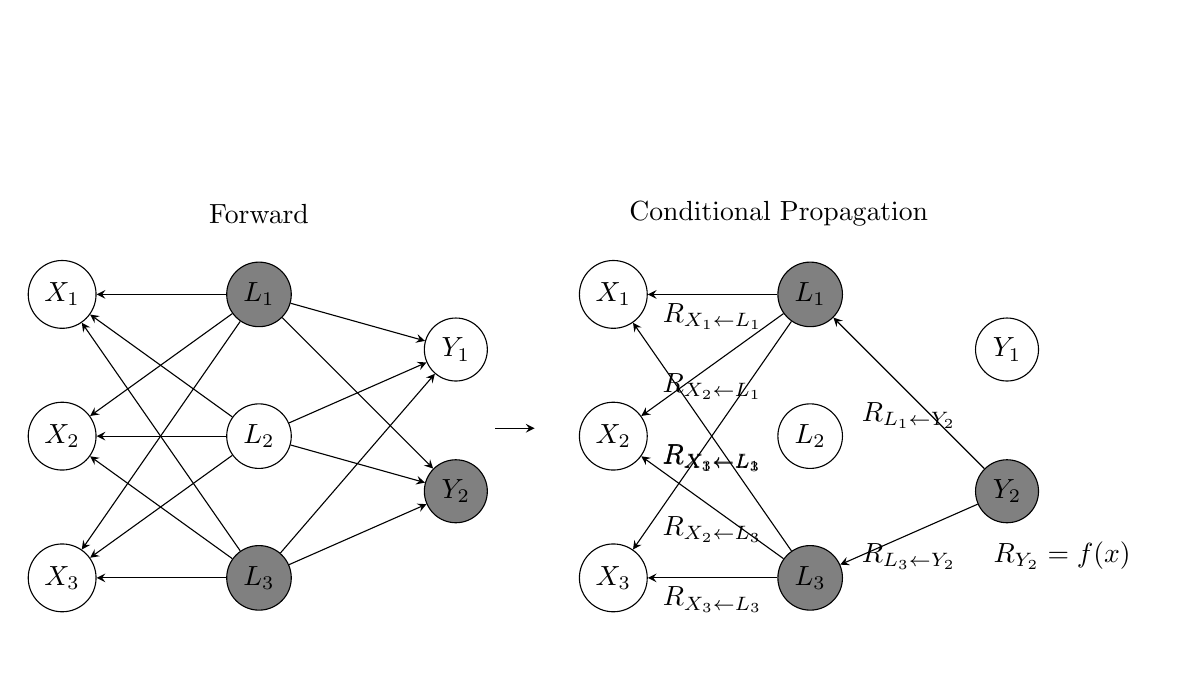
\begin{tikzpicture}[>=stealth,
            every node/.style={ draw, minimum size=8mm, align=center},]

        % First layer
        \foreach \x in {1,2,3} {
                \node [neuron] (X\x) at (0,{-\x* 1.8}) {$X_\x$};
            }
        \node [edgelabel]  (ti1) at (2.5,-0.5) {Forward};
        % Second layer
        \foreach \x in {1,2,3}{
                \pgfmathparse{\x==1 || \x ==3}
                \ifnum \pgfmathresult=1
                    \node  [neuron, conditioned]  (L\x) at (2.5,{-\x* 1.8}) {$L_\x$};
                \else
                    \node  [neuron]  (L\x) at (2.5,{-\x* 1.8}) {$L_\x$};
                \fi
            }

        % Last layer
        \foreach \x in {1,2} {
                \ifnum \x = 2
                    \node [neuron, conditioned]  (Y\x) at (5,{-\x* 1.8 - 0.7}) {$Y_\x$};
                    %\node [neuronlabel] at (Y\x.south) {$R_{Y_\x} = f(x)$};
                \else
                    \node  [neuron]  (Y\x) at (5,{-\x* 1.8 - 0.7}){$Y_\x$};
                \fi
            }

        % Connect nodes
        \foreach \y in {1,2,3}
        \foreach \x in {1,2,3}{
                \ifnum\x=\y
                    \draw[<-] (X\x) -- (L\y);
                    %node[midway, edgelabel] {$R_{X_\x  \gets L\y}$};
                \else
                    \pgfmathparse{2 > \x-\y && 2 > \y-\x}
                    \ifthenelse{\pgfmathresult=1}{\draw[<-] (X\x) -- (L\y);}{}
                \fi
            }
        \foreach \x in {1,2,3}
        \foreach \y in {1,2}
        \draw[->] (L\x) -- (Y\y);

        \draw[->] (5.5,-3.5) -- (6,-3.5);

        % OTHER GRAPH
        % First layer
        \foreach \x in {1,2,3} {
                \node [neuron] (X\x) at (7,{-\x* 1.8}) {$X_\x$};
            }

        % Second layer
        \node [edgelabel]  (ti2) at (9.1,-0.5) {Conditional Propagation};
        \foreach \x in {1,2,3}{
                \pgfmathparse{\x==1 || \x ==3}
                \ifnum \pgfmathresult=1
                    \node  [neuron, conditioned]  (L\x) at (9.5,{-\x* 1.8}) {$L_\x$};
                \else
                    \node  [neuron]  (L\x) at (9.5,{-\x* 1.8}) {$L_\x$};
                \fi
            }

        % Last layer
        \foreach \x in {1,2} {
                \ifnum \x = 2
                    \node [neuron, conditioned]  (Y\x) at (12,{-\x* 1.8 - 0.7}) {$Y_\x$};
                    \node [neuronlabel] at (12.7,{-\x* 1.8 - 1.3}) {$R_{Y_\x} = f(x)$};
                \else
                    \node  [neuron]  (Y\x) at (12,{-\x* 1.8 - 0.7}){$Y_\x$};
                \fi
            }

        % Connect nodes
        \foreach \y in {1,3}
        \foreach \x in {1,2,3}{
                \pgfmathparse{2 > \x-\y && 2 > \y-\x}
                \ifthenelse{\pgfmathresult=1}{\draw[<-] (X\x) -- (L\y)  node[midway, edgelabel] {$R_{X_\x  \gets L_\y}$};}{}
            }
        \foreach \x in {1,3}
        \foreach \y in {2}
        \draw[<-] (L\x) -- (Y\y) node[midway,align=center, edgelabel] {$R_{L_\x  \gets Y_\y}$};
    \end{tikzpicture}

    \caption[CRP Intuition]{\textbf{CRP Intuition:} Left side: simple neural network forward pass with input layer X, one hidden layer L and output layer Y. Conditioning set $\theta = \{L_1, L_3, Y_2\}$ \\ Right side: only the relevance of the neurons matching the conditioning set is propagated back \\
        Result at input pixel $R_{X_2} = \sum_{j}  R_{X_2 \gets L_j} =  \sum_i \sum_{j} \cdot \frac{a_i w_{ij}}{\sum_h a_h w_{hj}} R_j \dots$ }
    \label{fig:crp_example_condition}
\end{figure}

\subsubsection{Interpretation Techniques}

Heatmaps produced by conditional attribution could be analyzed in a similar fashion to the traditional class-specific heatmaps produced by LRP. The hindrance is that the meanings of the conditioned on latent features are not known, so it is unclear how to interpret the importance of some pixels for feature $i$ in layer $l$. For large, complex models some human-understandable concepts can emerge in hidden layers from simpler more local concepts in earlier and more abstract concepts in later layers \cite{Bau2017, Hohman2020, Olah2017, Bau2020}. However this is not a fact to rely on and seems to regularly fail for smaller models or simpler problems as noted before and in other work \todo{cite}.

CRP's authors therefore construct a framework for the understanding of these latent features. \textit{Activation Maximization} is used to find the samples for which the neuron (set) of a concept has the highest activation. They build on the idea of activation maximization when proposing \textit{Relevance Maximization}, where samples maximize the conditional relevance of a concept instead of the activation. Both methods yield a set of images or samples (see \autoref{fig:act_rel_max}), which can be enhanced further by masking out the irrelevant parts of the image, creating class specific reference samples and carefully selecting or extending the pool of samples to choose from. 

talk about Band-aid usage scenario, which is kinda "watermark" scenario. Why is the "perturbation" of activations / filters not a good idea? or is it?

is more of a \textit{human-in-the-loop} approach for finding/ removing Clever-Hans features. Example of actual watermark
\begin{quote}
From the graph, it can be inferred that the Clever Hans filters help the model in prediction, but they are not decisive for correct classification. Thus, the model relies on other potential non-Clever Hans features to detect the safe verifying the correct functioning of the model in cases of samples without watermarks.
\end{quote}

\begin{figure}[htbp]
    \centering
	\includegraphics[width=0.7\textwidth]{thesis_latex_template/pics/act_vs_relmax.png}
    \caption[ActMax vs. RelMax]{Activation Maximization in Comparison to Relevance Maximization. The image is cropped to the region with highest activation/relevance. }
    \label{fig:act_rel_max}
\end{figure}
\todo{image of ActMax and RelMax examples (using my dataset?)}

The resulting interpretation tools for single concepts are combined with methods for a local explanation, i.e. the analysis of a single sample or image. A \textit{Concept Atlas} (\cref{fig:attr_graph}) inspired by Carter et. al.'s \textit{Activation Atlas} \todo{cite} colors parts of an image based on the most relevant concept in that region. \textit{Hierarchical attribution graphs} (\cref{fig:attr_graph}) decompose the relevant concepts for an image into their lower layer sub-concept channels. The presumption being that the spread of relevance into lower level features helps in the understanding of relevant concepts for a sample.

\begin{figure}[htpb]
    \centering  
  \begin{minipage}[t]{0.45\textwidth}
  \vspace{-\topskip}
	\includegraphics[width=\textwidth]{thesis_latex_template/pics/concept_atlas.png}
    \end{minipage}
  \begin{minipage}[t]{0.45\textwidth}
  \vspace{-\topskip}
	\includegraphics[width=\textwidth]{thesis_latex_template/pics/example_hierarchical_attribution.png}
    \end{minipage}
    \label{fig:attr_graph}
    \caption[Concept Atlas and Hierarchical Attribution Graph]{Concept Atlas and Hierarchical Attribution Graph for an image in our dataset, looking at the last convolutional layer. The result is not as easy to interpret as in the example used in the CRP paper}
\end{figure}



papers using, extending on, similar to, evaluating CRP
which papers have been published on this
\begin{itemize}
    \item global: Assessing Concept Similarity in Latent Space
    \item papers with crp and more global explanation / concept clustering stuff 
\cite{Vielhaben2022,Vielhaben2023,Dreyer2023,Dreyer2023a,Fel2023,Fel2023a,Pahde2023}
    \item user evaluation study of authors in next paper \cite{Achtibat2023}
    \item 
      \item reveal to revise: whole framework for XAI using CRP as one of the methods for concept/bias discovery \cite{Pahde2023}
      \item using CRP to identify and unlearn bias 'Right Reason Class Artifact Compensation (RR-ClArC)' \cite{Dreyer2023a}
      \item newest summary paper, saying basically the same thing as old one, but with a (not so great) human evaluation study \cite{Achtibat2023}
      \item disentangle representations, similar to PCA, uses LRP \cite{Chormai2022}
\end{itemize}

\section{Evaluation of XAI Methods}
The research on quantification and evaluation of XAI methods has increased with their rising popularity. 
Explainable AI method's purpose is to describe the decision strategies of a machine learning model to ensure it is safe and fair to deploy for an application. 
Unless we can guarantee that an explanation indeed accurately identifies \textit{why} a decision has been made, it can not be used as a justification.
The core problem of evaluation explanation methods is that there is no agreed upon, mathematical definition of a \textit{good} explanation. However, attempts to rigorously compare XAI methods have been made using proxies:\\

A successful explanation is not only correct (i.e. faithful to the model), but also sufficient, technically applicable and understandable by humans \cite{Samek2021}. Work on evaluating XAI methods can therefore be generally divided into these categories, with different metrics or experiments to measure respective performance. One can try to measure those factors on real problems, create benchmarks with known ground truth explanations or conduct human studies. Within these possibilities we focus on evaluation methods for local attribution methods, back-propagation methods and concept-based methods, applicable to our study subject \textit{CRP}.

\subsection{Fidelity, Correctness, Faithfulness}

Recently, a multitude of benchmarks and theoretical analyses have examined the fidelity, especially of local attribution methods, to the model they are trying to explain. Evaluations commonly used by authors of new XAI methods include feature ablation \cite{Samek2017} and data randomization (e.g. pixel flipping) \cite{Adebayo2018}. 
These metrics hypothesize that changing or removing the most important features from the input should significantly reduce the models ability to predict accurately.

While this does to some degree follow a causal idea, it ignores the generating factors which do not necessarily surface within single pixels and is prone to errors because the choice of a proper baseline is in itself a hard task as the true causal pathways in the data distribution are usually not known. Another issue is that removing the most important features does not necessarily remove their whole information, because the boundary of the image region might still resemble the removed object.
When choosing the baseline by averaging over the existing training set, one might introduce biases, but just greying out pixels is out of the distribution of true images too.

\cite{Bluecher2022}
- interactions of different concepts with each other
- close / similar to shapely values
-

\cite{Rong2022}
- eliminates problem that perturbing "important" pixels has information leakage as shape is visible
- ROAD
- new evaluation strategy for attribution methods: remove and debias


\subsection{Sensitivity, Sufficiency}
\cite{Wilming2023, Clark2023}



\paragraph*{XAI-TRIS:}
(could also fit into "with known ground truth importance" category)
\cite{Clark2023}
Gleich
\begin{itemize}
      \item similar "causal" model for benchmarks
      \item idea of signal-to-noise ratio style setup from here
\end{itemize}

Anders
\begin{itemize}
      \item they say suppressor variables should not be important. However if they have a causal effect on the model (which they do, cause prediction is worse without them) in our opinion they should be important.
      \item question is: what should the correct explanation be, when constant vector shift or out-of-distribution sample makes good prediction impossible?
      \item in my opinion: putting attention onto the suppressor feature is a good way to show that the model can't deal with it well
      \item Performance Metrics: Precision? / Earth Mover's Distance (Wasserstein) between binary gt and heatmap
\end{itemize}

\paragraph{Wilming, Suppressor Variables}
\cite{Wilming2023,Clark2023}
\begin{itemize}
    \item their experiment is based on the idea that a model explanation should be able to distinguish between a \textit{spurious} (in their case \textit{suppressor} feature and a \textit{core} feature. 
    \item in the simple model they create, $X_1$ is a collider for the core $Y$ and the other $X_2$ feature, so the SCM is not the same. But learning $X_2$ might still help.
    \item in our example, the other generating factors such as scale and rotation are similar to the suppressor variable they propose. 
    \item we believe that it would be strange to assume the model to assign 0 importance to those features, as they have to be learned to understand the model space
    \item While the explanation in our experiment is not independent of the other generating factors, in general the causal effect of changing these is magnitudes lower than changing the core or spuriously correlated features. 
    \item they only find methods which purposefully include the data distribution of the training data into the explanation to be successful
    \item we argue that, while getting insights into that, it does not explain what the \textbf{model} itself is doing.
    \item As we show in our experiment, the relationship between what is present in the data and what a model learns, while it generally follows a trend, is not exactly linear
    \item hence our title \textit{are we explaining the data or the model?}
    \item nothing wrong with explaining the underlying data too. but in application cases we don't have that information. Or we want good explanations independent on the data the model was trained on
\end{itemize}

\cite{Clark2023} on XAI papers: 
\begin{quote}
A recent survey showed that one in three XAI papers evaluate methods exclusively with anecdotal
evidence, and one in five with user studies Nauta et al. (2023). Other work in the field tends to
focus on secondary criteria (such as stability and robustness Rosenfeld et al. (2021-03-27); Hedström
et al. (2022)) or subjective or potentially circular criteria (such as fidelity and faithfulness Gevaert et al. (2022); Nauta et al. (2023)). We doubt that such validation approaches can fully replace metrics assessing objective notions of ‘correctness’ of explanations, considering that XAI methods are widely intended to be used as means of quality assurance for machine learning systems in critical applications.
\end{quote}

\subsection{Human Interpretability}
{\color{gray} 
evaluation studies, old notes:
\begin{enumerate}
      \item \cite{Sixt2022a}: evaluation of heatmaps/saliency methods not enough based on actual user studies and human performance / explanation quality
            \\ task: look at explanation and rate, weather each feature is relevant or irrelevant
            \textit{Similar to our work they investigate how well users can quantify biases of a model, one of the most important applications of XAI methods.}
      \item \cite{Wilming2023}: explanation of suppressor variables (that have no statistical association with target) gives false impression that of dependency if their inclusion into the model improves it
            \\ task: linear model with 1 real and 1 suppressor variable, saliency methods mark both suppressor variable and core variable as important
      \item \cite{Sixt2020}: because matrix is converging to rank 1 in BP methods that dont use negative relevance scores appropriately, heatmaps are not class sensitive
            \\ task: randomize more and more network parameters, look at heatmap for and against class
      \item \cite{Kindermans2019}: heatmap methods are sensitive to constant shift in input data, but should fulfill input invariance
            \\ task: add “watermark style” input shift, test if model still predicts accurately and then if heatmap does same as model
      \item \cite{Karimi2023}: explanation depends more on hyperparameters than on model weights and prediction itself
            \\ task: quantify treatment effect when changing hyperparameters in comparison to changing model weights
      \item \cite{Adebayo2018}: some saliency methods are independent to both the model and the data generating factors (not testing LRP)
            \\ task: compare explanation trained on true model with explanation trained with random labels, also compare to simple edge detector which is very similar often
      \item \cite{Sixt2022}: deep taylor decomposition fails, when only positive relevance taken into account, matrix falls to rank 1 \\ task: theoretical analysis
\end{enumerate}
}


From \cite{Yang2019}:
\begin{itemize}
    \item Sensitivity and Robustness: explanation changes same as model/output changes \cite{Adebayo2018,Ghorbani2019a}
    \item Correctness: e.g. feature ablation (=faithfulness, fidelity) \cite{Samek2017a,Fong2017,Hooker2019} Hooker use retraining, others don't
    \item with ground truth knowledge of feature importance \cite{Kim2018, Yang2019, Clark2023,Arras2022,Bau2017,Parafita2019,Singla2022}
    \item with humans in the loop \cite{Singla2022, Ribeiro2016, Rong2023,Kim2018}
\end{itemize}

From \cite{Samek2021}:
\begin{itemize}
    \item Faithfulness/Sufficiency: 'pixel-flipping' \cite{Samek2017}
    \item Human Interpretability \cite{Kim2018}, file size of explanation
    \item Applicability and Runtime
\end{itemize}

From \cite{Arras2022}:
\begin{itemize}
    \item Pixel Perturbation == feature ablation pixel flipping \cite{Samek2017a, Samek2021, Bach2015, Lundberg2017}
    \item Data Randomization \cite{Adebayo2018}
    \item Model Randomization \cite{Adebayo2018,Sixt2020}
    \item Remove and Retrain \cite{Hooker2019}
    \item Object Localization / Segmentation \cite{Simonyan2014}
    \item Pointing Game
\end{itemize}


\subsection{With Known Ground Truth}
Additionally, more complex benchmarks \cite{Kim2018, Arras2022, Bau2017, Singla2022} which are often human-supervised aim at comparing XAI outputs to human-understandable concepts.

In the quantitative evaluation of \cite{Kim2018} a similar approach to ours is put into action:
a noise parameter controls the correlation of an image and a label on it and the accuracy for images without the label is tested. If the label was not learned as an important feature, the TCAV score should be low. User studies showed that saliency maps for TCAVs did not help in identifying the important feature. This is an important insight and corresponds with \cite{Sixt2022a}. It seems that saliency maps are misleading more often than not. If there is no additional insight as with CRPs relevance images or similar, one can not expect to tell spurious from core features only using saliency maps.

\begin{itemize}
      \item examples of often used evaluations for local attribution methods and concept-based methods:
            \begin{itemize}
                  \item feature ablation and related methods
                  \item TCAVs \cite{Kim2018} with benchmark feature set (hard and often not applicable)
                  \item clevr-xai? \cite{Arras2022}
            \end{itemize}
      \item clever XAI artificial benchmark dataset \cite{Arras2022}
      \item NetDissect dataset with concept-segmented images \cite{Bau2017}
      \item also other concept/neuron dissection by same authors, similar idea to CRP \cite{Bau2020}
      \item creates new dataset (human-supervised) to detect core vs spurious features \cite{Singla2022}
\end{itemize}

\cite{Yang2019}
- Common Feature Measure -> how many of the (10) classes have this feature in background (e.g. dog)
- vary cf measure from 0.1 (only one class has feature = watermark) to 0.9 (9 out of 10 classes have feature)
- measure MCS = Model Contrast Score = how different is importance of cf in different models

\cite{Arras2022}
- clevr-xai = known ground truth importance
- Mass Accuracy = relevance within feature bounding box / total relevance in image
- Rank Accuracy = how many of the pixels inside bounding box are in K most important pixels


{\color{red} outline which problems CRP solves well, draw connections between unsolved criticism and causal perspective}

Although a general lack of dependence between explanations and their model \cite{Adebayo2018,Karimi2023} has so far only been studied for attribution methods that are not concept-based, current research still draws a less than ideal picture of their fidelity.
Kindermans et al. \cite{Kindermans2019} show that a constant vector shift on the input data, which is not affecting the performance of the model, can lead to misleading explanations. The theoretical and empirical analysis of \cite{Sixt2020} finds the class insensitivity of some back-propagation methods to be due to their improper use of negative relevance.
While authors of new methods often underline their applicability with user studies \cite{Achtibat2023,Fel2023,Ghorbani2019,Zhang2021}, Sixt et al. \cite{Sixt2022a} among others \cite{Singla2022} show that XAI methods do not necessarily increase humans skill at identifying relevant features. Similarly, Rong et al. \cite{Rong2023} criticizes a lack of comparability between user studies in the field of XAI. 

Constructing an evaluation test which is neither too simple and therefore too far away from realistic application scenarios nor not quantifiable empirically due to its \textit{human} component or unidentifiable ground truth, poses a challenge which \cite{Clark2023} tries to tackle. This benchmark is based on recent analysis \cite{Wilming2023} of suppressor variables, which can be for example the background color of an image, that are used by the model without having an association to the core features to normalize the image and improve the prediction.
They introduce a generation process for mixing the suppressor and real features which serves as inspiration for the structural causal model applied in our case.

\begin{itemize}
      \item explanations are independent of later layers (no negative relevance) \cite{Sixt2020}
      \item suppressor variable "in practice, XAI methods do not distinguish whether a feature is a confounder or a suppressor, which can lead to misunderstandings about a model's performance and interpretation"
      \item kinda stupid, because neural network also does not make a difference between suppressors and confounders \cite{Wilming2023}
      \item the (un-)reliability of saliency methods: should fulfill 'input invariance'
      \item saliency method mirrors sensitivity of model with respect to transformations of the input
      \item normal LRP root point (zero) not working
      \item pattern attribution reference point works (direction of variation in data, determined by covariances) \cite{Kindermans2019}
\end{itemize}


\section{Causal Inference}
In the following we summarize the causal inference and estimation framework used for our analysis. 
Although the principles of causality seem to be innate in human rational thinking, they have been formalized not so long ago \cite{Spirtes1993, Halpern2005, Pearl2000} and efforts to include causal notions into fields like AI have also been met with doubts and caution. 

\subsection{Ladder of Causation}
As mentioned before, most machine learning methods including deep neural networks do not attempt to learn causal relationships but merely \textit{associations}. These are on the first ladder of causation as described by Pearl \cite{Pearl2000}. Many explanation methods do not go beyond the statistical associations as found in the models output either and ask questions like \textit{How does seeing prediction Y change my believe that X is important}. However in recent years there has been an effort to climb the ladder of causation and answer \textit{what if} questions like \textit{how does the model output Y change if I change X} by creating \textit{interventions} on the input or the model parameters. The highest rank of causation, \textit{counterfactuals}, answers \textit{why} questions. One concrete example would be: \textit{How would the output Y have changed, if X had been different}. 

\subsection{Structural Causal Models}
To analyze and quantify causal relationships, \textit{structural causal models} are defined, based on the observable variables \textbf{X}, the unobserved or noise variables \textit{U} and their probability distribution $P_u$, and structural assignments \textit{f}. The structural assignments represent causal mechanisms between a variable $x_i$ and its parents $Pa(x_i) \in (X \setminus \{x_i\}) \cup U$  such that $\forall x_i \in X, x_i = f_i(Pa(x_i),u_i)$. 
Structural causal models, or short SCMs, can be represented by a directed acyclic graph (DAG) $G(V,E)$ known as a causal Bayesian network. The nodes $V$ are the endogenous (or observable) variables and the directed edges represent the causal mechanisms $f$ from each parent variable in $PA^i$ to its child $x_i$. We assume that \textit{structural minimality} holds for the SCM and its graph, which means that if a directed edge between two variables X and Y exists, there is a non-zero causal effect from X to Y. 
In general the structural assignments $f$ can take any shape, though restricted SCMs pose assumptions on the type of functions possible. Importantly, if no assumptions are made, the direction of causal links is not always identifiable \cite{Peters2017}. Even though in practice one can for example often assume that the noise is not exactly Gaussian, which makes identification possible, this is not necessarily the case for complex image data. As we will see later, the directions of causal links cannot be easily identified for typical image classification tasks and this shall not be the goal of this work. By generating a toy dataset with a predefined SCM we can estimate causal effects because the causal directions are known.

Something about \textit{independent mechanisms}

\subsection{Causal Effect Estimation}
A hard intervention on a variable $X$, denoted as $do(X := x_0)$ is replacing the previous structural assignment of that variable ($X = f(PA_x, \eta_x)$) with a fixed value $x_0$.  
In the associated causal graph this is equivalent to removing all in-going edges of $X$.
When the causal model is at least partly known, causal effects can be estimated by intervention. The average causal effect of a binary variable $X$ on another variable $Y$ is defined as follows:

\begin{equation}
\displaystyle ACE = \mathbb{E} [ y \ | \ do(x=1) ] - \mathbb{E} [ y \ | \ do(x=0) ] 
\end{equation}
In recent years a multitude of work has taken variants of this average causal effect and of SCMs to either explain AI models directly or to evaluate explanations. 

\section{Towards More Causal Evaluation of XAI}\label{section:causal_xai}

There is a long-standing relationship between causality and AI research and explaining a models decision is in itself a causal task.
As Schölkopf argues, ''the hard open problems of machine learning and AI are intrinsically related to causality'' \cite{Schoelkopf2019}.
Built on a philosophical and theoretical foundation \cite{Woodward2004, Halpern2005, Schoelkopf2019} many authors have already started using more causal language when describing the goals of explanation methods. Moraffah et al. \cite{Moraffah2020a} survey current causal XAI methods as well as causal evaluation of XAI methods. Beckers \cite{Beckers2022} formally defines \textit{sufficient} and \textit{counterfactual explanations} as well as \textit{actual causation} in the 'action-guiding' setting that is XAI. He argues that a good explanation not only shows which things ought to be changed for a different outcome but also makes clear which ''\textit{may not be manipulated}''. In computer vision tasks there is no standard way of explaining the contextual data distribution that ought to stay fixed. 

There is therefore a growing variance of generating counterfactual explanations \cite{Moraffah2020a}. Similarly, feature attribution needs to make decisions on how to explain in the context of the training distribution. 
Some authors \cite{Kindermans2017,Wilming2023, Wilming2022} argue, that explanation methods should learn to ignore the underlying data distribution with potential spurious correlations by incorporating it into the explanation process. Others believe that one of the core use-cases of explanation methods is to uncover these \textit{Clever-Hans} artifacts, stemming from skewed training distributions. It seems not advisable to apply a biased model to an out-of-distribution scenario, even though the learned spurious features (or suppressor variables) might not have an effect on the outcome (yet).\\

Causal methods can be applied in multiple ways in a prediction/explanation setting.
Some authors use more fine-grained features like single pixels as implicit causal variables, especially for scenarios without a known ground truth importance \cite{Zeiler2013,Fong2017,Samek2017a}. Others use known ground truth factors or learn abstract concepts as causal variables in an unsupervised manner \cite{Goyal2019, Tran2022, Reimers2019, Reimers2020, Harradon2018}. The third approach is to interpret the neural network itself as a causal graph and hidden neurons as causal variables that can be intervened on \cite{Narendra2018, Chattopadhyay2019}. Karimi et al. \cite{Karimi2023} on the other hand, interpret the whole process from hyperparameters to the explanation as one causal model and intervene on model hyperparameters. 
In all cases, the goal is to estimate the effect of interventions on the model prediction and explanation, either to construct a new (counterfactual) explanation method or to evaluate existing methods.
Our work in principle also intervenes on a variable in order to measure causal effects. Similar to Karimi et al. \cite{Karimi2023} our variable can be seen as a hyperparameter to the whole model training and explanation generation process and we do not aim to generate explanations but study their relationship with the prediction. In their work, they intervene on many training hyperparameters in order to compare the influence on the prediction to the influence on the explanation. Their hypothesis is that a good explanation should be determined only by the prediction and therefore the effects of the hyperparameters on the explanation should be completely mediated by the prediction. By carefully constructing a process where only one variable in a data distribution changes, we conduct a similar experiment. 


\subsection{Interpreting The Explanation Process as a Causal Model}

\begin{itemize}
    \item observational study looking at real world correlated datasets disentanglement, correlated things are not properly disentangled \cite{Traeuble2021} 
\end{itemize}

 \cite{Yang2019} Benchmarking attribution methods with relative feature importance


